\documentclass{standalone}
\usepackage{tikz}
\usetikzlibrary{patterns, positioning}

\begin{document}
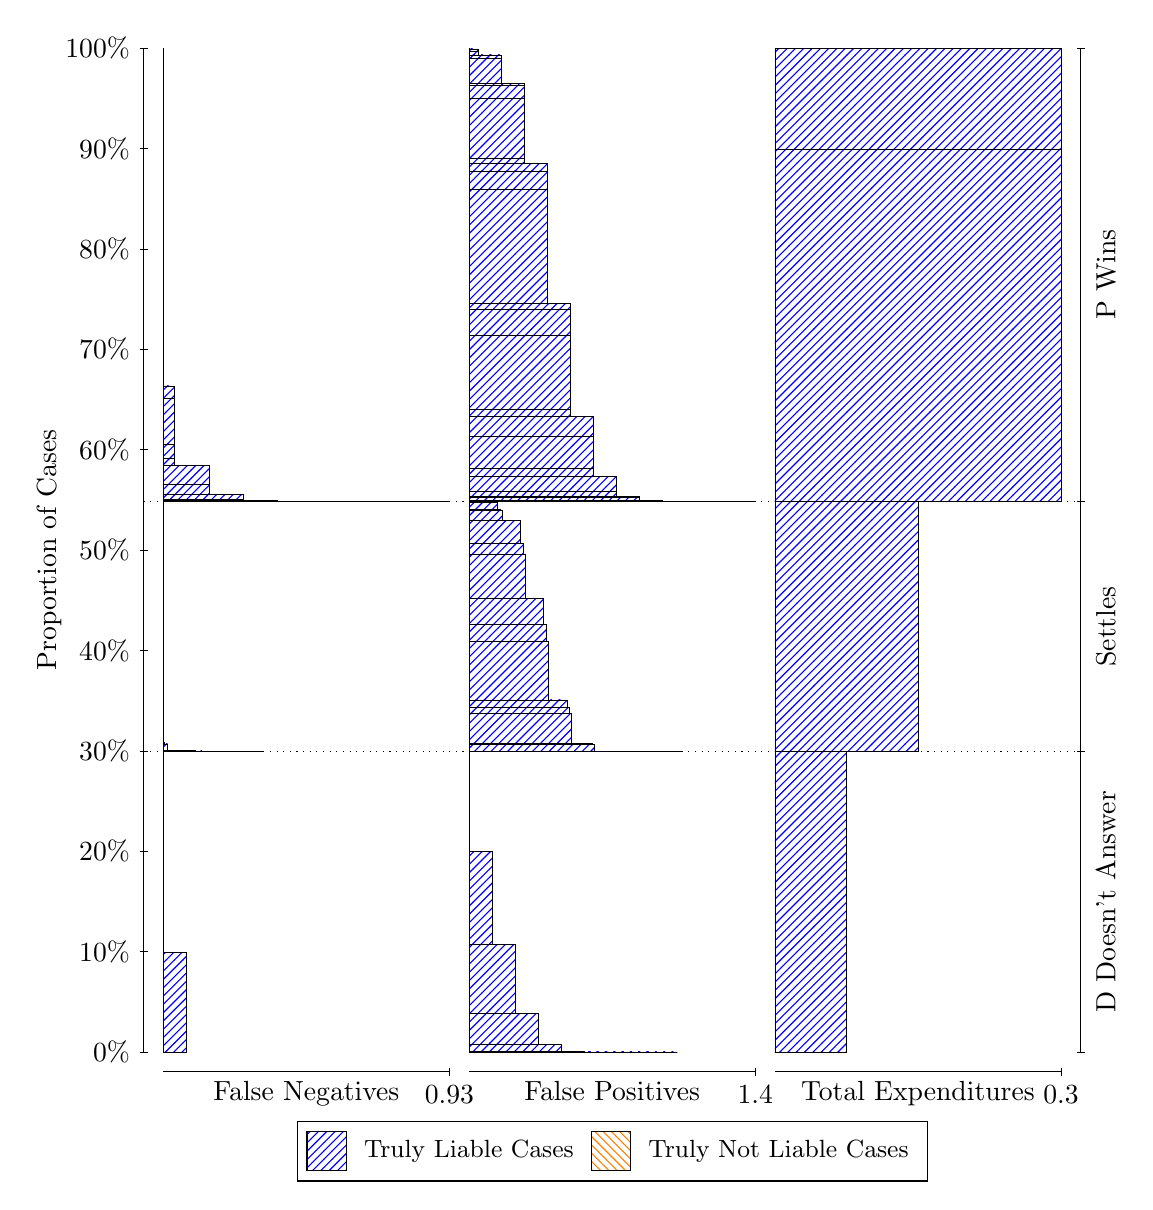
\begin{tikzpicture}
\draw[black, very thin] (1.5,1.75) -- (1.5,14.5);
\node[rotate=90, anchor=center] at (0.3, 8.125) {Proportion of Cases};
\draw[black, very thin] (1.45,1.75) -- (1.55,1.75);
\node[anchor=east] at (1.45, 1.75) {0\%};
\draw[black, very thin] (1.45,3.025) -- (1.55,3.025);
\node[anchor=east] at (1.45, 3.025) {10\%};
\draw[black, very thin] (1.45,4.3) -- (1.55,4.3);
\node[anchor=east] at (1.45, 4.3) {20\%};
\draw[black, very thin] (1.45,5.575) -- (1.55,5.575);
\node[anchor=east] at (1.45, 5.575) {30\%};
\draw[black, very thin] (1.45,6.85) -- (1.55,6.85);
\node[anchor=east] at (1.45, 6.85) {40\%};
\draw[black, very thin] (1.45,8.125) -- (1.55,8.125);
\node[anchor=east] at (1.45, 8.125) {50\%};
\draw[black, very thin] (1.45,9.4) -- (1.55,9.4);
\node[anchor=east] at (1.45, 9.4) {60\%};
\draw[black, very thin] (1.45,10.675) -- (1.55,10.675);
\node[anchor=east] at (1.45, 10.675) {70\%};
\draw[black, very thin] (1.45,11.95) -- (1.55,11.95);
\node[anchor=east] at (1.45, 11.95) {80\%};
\draw[black, very thin] (1.45,13.225) -- (1.55,13.225);
\node[anchor=east] at (1.45, 13.225) {90\%};
\draw[black, very thin] (1.45,14.5) -- (1.55,14.5);
\node[anchor=east] at (1.45, 14.5) {100\%};

\draw[black, very thin] (13.4,1.75) -- (13.4,14.5);
\draw[black, very thin] (13.35,1.75) -- (13.45,1.75);
\node[anchor=west] at (13.35, 1.75) {};
\draw[black, very thin] (13.35,5.5631) -- (13.45,5.5631);
\node[anchor=west] at (13.35, 5.5631) {};
\draw[black, very thin] (13.35,8.7449) -- (13.45,8.7449);
\node[anchor=west] at (13.35, 8.7449) {};
\draw[black, very thin] (13.35,14.5) -- (13.45,14.5);
\node[anchor=west] at (13.35, 14.5) {};

\draw[black, very thin, pattern color=blue, pattern=north east lines] (1.75,1.75) rectangle (2.0446,3.0136);
\draw[black, very thin, pattern color=orange, pattern=north west lines] (1.75,3.0136) rectangle (1.75,3.0136);
\draw[black, very thin, pattern color=blue, pattern=north east lines] (1.75,3.0136) rectangle (1.75,5.5631);
\draw[black, very thin, pattern color=blue, pattern=north east lines] (1.75,5.5631) rectangle (3.0266,5.5631);
\draw[black, very thin, pattern color=blue, pattern=north east lines] (1.75,5.5631) rectangle (2.6338,5.5631);
\draw[black, very thin, pattern color=blue, pattern=north east lines] (1.75,5.5631) rectangle (2.5901,5.5631);
\draw[black, very thin, pattern color=blue, pattern=north east lines] (1.75,5.5631) rectangle (2.241,5.5741);
\draw[black, very thin, pattern color=blue, pattern=north east lines] (1.75,5.5741) rectangle (2.1973,5.5747);
\draw[black, very thin, pattern color=blue, pattern=north east lines] (1.75,5.5747) rectangle (2.1537,5.5804);
\draw[black, very thin, pattern color=blue, pattern=north east lines] (1.75,5.5804) rectangle (1.8046,5.6627);
\draw[black, very thin, pattern color=blue, pattern=north east lines] (1.75,5.6627) rectangle (1.7609,5.6835);
\draw[black, very thin, pattern color=orange, pattern=north west lines] (1.75,5.6835) rectangle (1.75,5.6835);
\draw[black, very thin, pattern color=blue, pattern=north east lines] (1.75,5.6835) rectangle (1.75,8.7449);
\draw[black, very thin, pattern color=blue, pattern=north east lines] (1.75,8.7449) rectangle (5.3833,8.7449);
\draw[black, very thin, pattern color=blue, pattern=north east lines] (1.75,8.7449) rectangle (4.9469,8.7449);
\draw[black, very thin, pattern color=blue, pattern=north east lines] (1.75,8.7449) rectangle (4.5105,8.7449);
\draw[black, very thin, pattern color=blue, pattern=north east lines] (1.75,8.7449) rectangle (4.5105,8.7449);
\draw[black, very thin, pattern color=blue, pattern=north east lines] (1.75,8.7449) rectangle (4.074,8.7449);
\draw[black, very thin, pattern color=blue, pattern=north east lines] (1.75,8.7449) rectangle (3.6376,8.7455);
\draw[black, very thin, pattern color=blue, pattern=north east lines] (1.75,8.7455) rectangle (3.6376,8.7458);
\draw[black, very thin, pattern color=blue, pattern=north east lines] (1.75,8.7458) rectangle (3.2012,8.7555);
\draw[black, very thin, pattern color=blue, pattern=north east lines] (1.75,8.7555) rectangle (2.7647,8.7713);
\draw[black, very thin, pattern color=blue, pattern=north east lines] (1.75,8.7713) rectangle (2.7647,8.8331);
\draw[black, very thin, pattern color=blue, pattern=north east lines] (1.75,8.8331) rectangle (2.3283,8.9607);
\draw[black, very thin, pattern color=blue, pattern=north east lines] (1.75,8.9607) rectangle (2.3283,9.1981);
\draw[black, very thin, pattern color=blue, pattern=north east lines] (1.75,9.1981) rectangle (1.8918,9.2858);
\draw[black, very thin, pattern color=blue, pattern=north east lines] (1.75,9.2858) rectangle (1.8918,9.474);
\draw[black, very thin, pattern color=blue, pattern=north east lines] (1.75,9.474) rectangle (1.8918,10.055);
\draw[black, very thin, pattern color=blue, pattern=north east lines] (1.75,10.055) rectangle (1.8918,10.209);
\draw[black, very thin, pattern color=orange, pattern=north west lines] (1.75,10.209) rectangle (1.75,10.209);
\draw[black, very thin, pattern color=blue, pattern=north east lines] (1.75,10.209) rectangle (1.75,14.5);
\draw[black, very thin, pattern color=orange, pattern=north west lines] (5.6333,1.75) rectangle (8.2758,1.75);
\draw[black, very thin, pattern color=blue, pattern=north east lines] (5.6333,1.75) rectangle (8.2758,1.75);
\draw[black, very thin, pattern color=blue, pattern=north east lines] (5.6333,1.75) rectangle (7.9822,1.75);
\draw[black, very thin, pattern color=blue, pattern=north east lines] (5.6333,1.75) rectangle (7.6886,1.75);
\draw[black, very thin, pattern color=blue, pattern=north east lines] (5.6333,1.75) rectangle (7.3949,1.7503);
\draw[black, very thin, pattern color=blue, pattern=north east lines] (5.6333,1.7503) rectangle (7.1013,1.7582);
\draw[black, very thin, pattern color=blue, pattern=north east lines] (5.6333,1.7582) rectangle (6.8077,1.8434);
\draw[black, very thin, pattern color=blue, pattern=north east lines] (5.6333,1.8434) rectangle (6.5141,2.2366);
\draw[black, very thin, pattern color=blue, pattern=north east lines] (5.6333,2.2366) rectangle (6.2205,3.1157);
\draw[black, very thin, pattern color=blue, pattern=north east lines] (5.6333,3.1157) rectangle (5.9269,4.2995);
\draw[black, very thin, pattern color=blue, pattern=north east lines] (5.6333,4.2995) rectangle (5.6333,5.5631);
\draw[black, very thin, pattern color=orange, pattern=north west lines] (5.6333,5.5631) rectangle (8.3418,5.5631);
\draw[black, very thin, pattern color=blue, pattern=north east lines] (5.6333,5.5631) rectangle (8.3418,5.5631);
\draw[black, very thin, pattern color=orange, pattern=north west lines] (5.6333,5.5631) rectangle (8.0776,5.5631);
\draw[black, very thin, pattern color=blue, pattern=north east lines] (5.6333,5.5631) rectangle (8.0776,5.5631);
\draw[black, very thin, pattern color=blue, pattern=north east lines] (5.6333,5.5631) rectangle (8.0482,5.5631);
\draw[black, very thin, pattern color=orange, pattern=north west lines] (5.6333,5.5631) rectangle (7.8133,5.5631);
\draw[black, very thin, pattern color=blue, pattern=north east lines] (5.6333,5.5631) rectangle (7.8133,5.5635);
\draw[black, very thin, pattern color=blue, pattern=north east lines] (5.6333,5.5635) rectangle (7.784,5.5635);
\draw[black, very thin, pattern color=blue, pattern=north east lines] (5.6333,5.5635) rectangle (7.7546,5.5635);
\draw[black, very thin, pattern color=blue, pattern=north east lines] (5.6333,5.5635) rectangle (7.5197,5.572);
\draw[black, very thin, pattern color=blue, pattern=north east lines] (5.6333,5.572) rectangle (7.4904,5.5723);
\draw[black, very thin, pattern color=blue, pattern=north east lines] (5.6333,5.5723) rectangle (7.461,5.5723);
\draw[black, very thin, pattern color=blue, pattern=north east lines] (5.6333,5.5723) rectangle (7.2261,5.6577);
\draw[black, very thin, pattern color=blue, pattern=north east lines] (5.6333,5.6577) rectangle (7.1968,5.6653);
\draw[black, very thin, pattern color=blue, pattern=north east lines] (5.6333,5.6653) rectangle (7.1674,5.6704);
\draw[black, very thin, pattern color=blue, pattern=north east lines] (5.6333,5.6704) rectangle (6.9325,6.0536);
\draw[black, very thin, pattern color=blue, pattern=north east lines] (5.6333,6.0536) rectangle (6.9032,6.1257);
\draw[black, very thin, pattern color=blue, pattern=north east lines] (5.6333,6.1257) rectangle (6.8738,6.2208);
\draw[black, very thin, pattern color=blue, pattern=north east lines] (5.6333,6.2208) rectangle (6.6389,6.964);
\draw[black, very thin, pattern color=blue, pattern=north east lines] (5.6333,6.964) rectangle (6.6096,7.1771);
\draw[black, very thin, pattern color=blue, pattern=north east lines] (5.6333,7.1771) rectangle (6.5802,7.5148);
\draw[black, very thin, pattern color=blue, pattern=north east lines] (5.6333,7.5148) rectangle (6.3453,8.0655);
\draw[black, very thin, pattern color=blue, pattern=north east lines] (5.6333,8.0655) rectangle (6.316,8.2162);
\draw[black, very thin, pattern color=blue, pattern=north east lines] (5.6333,8.2162) rectangle (6.2866,8.5055);
\draw[black, very thin, pattern color=blue, pattern=north east lines] (5.6333,8.5055) rectangle (6.0517,8.6244);
\draw[black, very thin, pattern color=blue, pattern=north east lines] (5.6333,8.6244) rectangle (6.0224,8.6453);
\draw[black, very thin, pattern color=blue, pattern=north east lines] (5.6333,8.6453) rectangle (5.993,8.7275);
\draw[black, very thin, pattern color=blue, pattern=north east lines] (5.6333,8.7275) rectangle (5.7581,8.7333);
\draw[black, very thin, pattern color=blue, pattern=north east lines] (5.6333,8.7333) rectangle (5.7288,8.7338);
\draw[black, very thin, pattern color=blue, pattern=north east lines] (5.6333,8.7338) rectangle (5.6994,8.7448);
\draw[black, very thin, pattern color=blue, pattern=north east lines] (5.6333,8.7448) rectangle (5.6333,8.7449);
\draw[black, very thin, pattern color=orange, pattern=north west lines] (5.6333,8.7449) rectangle (9.2667,8.7449);
\draw[black, very thin, pattern color=blue, pattern=north east lines] (5.6333,8.7449) rectangle (9.2667,8.7449);
\draw[black, very thin, pattern color=orange, pattern=north west lines] (5.6333,8.7449) rectangle (8.9731,8.7449);
\draw[black, very thin, pattern color=blue, pattern=north east lines] (5.6333,8.7449) rectangle (8.9731,8.7449);
\draw[black, very thin, pattern color=orange, pattern=north west lines] (5.6333,8.7449) rectangle (8.6795,8.7449);
\draw[black, very thin, pattern color=blue, pattern=north east lines] (5.6333,8.7449) rectangle (8.6795,8.7449);
\draw[black, very thin, pattern color=blue, pattern=north east lines] (5.6333,8.7449) rectangle (8.3859,8.745);
\draw[black, very thin, pattern color=orange, pattern=north west lines] (5.6333,8.745) rectangle (8.3859,8.745);
\draw[black, very thin, pattern color=blue, pattern=north east lines] (5.6333,8.745) rectangle (8.3859,8.7456);
\draw[black, very thin, pattern color=orange, pattern=north west lines] (5.6333,8.7456) rectangle (8.0923,8.7456);
\draw[black, very thin, pattern color=blue, pattern=north east lines] (5.6333,8.7456) rectangle (8.0923,8.7497);
\draw[black, very thin, pattern color=blue, pattern=north east lines] (5.6333,8.7497) rectangle (8.0923,8.7512);
\draw[black, very thin, pattern color=blue, pattern=north east lines] (5.6333,8.7512) rectangle (8.0923,8.7531);
\draw[black, very thin, pattern color=orange, pattern=north west lines] (5.6333,8.7531) rectangle (7.7987,8.7531);
\draw[black, very thin, pattern color=blue, pattern=north east lines] (5.6333,8.7531) rectangle (7.7987,8.7971);
\draw[black, very thin, pattern color=blue, pattern=north east lines] (5.6333,8.7971) rectangle (7.7987,8.8077);
\draw[black, very thin, pattern color=blue, pattern=north east lines] (5.6333,8.8077) rectangle (7.5051,8.8656);
\draw[black, very thin, pattern color=orange, pattern=north west lines] (5.6333,8.8656) rectangle (7.5051,8.8656);
\draw[black, very thin, pattern color=blue, pattern=north east lines] (5.6333,8.8656) rectangle (7.5051,9.063);
\draw[black, very thin, pattern color=blue, pattern=north east lines] (5.6333,9.063) rectangle (7.2114,9.162);
\draw[black, very thin, pattern color=orange, pattern=north west lines] (5.6333,9.162) rectangle (7.2114,9.162);
\draw[black, very thin, pattern color=blue, pattern=north east lines] (5.6333,9.162) rectangle (7.2114,9.5646);
\draw[black, very thin, pattern color=blue, pattern=north east lines] (5.6333,9.5646) rectangle (7.2114,9.8178);
\draw[black, very thin, pattern color=blue, pattern=north east lines] (5.6333,9.8178) rectangle (6.9178,9.9142);
\draw[black, very thin, pattern color=orange, pattern=north west lines] (5.6333,9.9142) rectangle (6.9178,9.9142);
\draw[black, very thin, pattern color=blue, pattern=north east lines] (5.6333,9.9142) rectangle (6.9178,10.846);
\draw[black, very thin, pattern color=blue, pattern=north east lines] (5.6333,10.846) rectangle (6.9178,11.185);
\draw[black, very thin, pattern color=blue, pattern=north east lines] (5.6333,11.185) rectangle (6.9178,11.255);
\draw[black, very thin, pattern color=orange, pattern=north west lines] (5.6333,11.255) rectangle (6.6242,11.255);
\draw[black, very thin, pattern color=blue, pattern=north east lines] (5.6333,11.255) rectangle (6.6242,12.708);
\draw[black, very thin, pattern color=blue, pattern=north east lines] (5.6333,12.708) rectangle (6.6242,12.941);
\draw[black, very thin, pattern color=blue, pattern=north east lines] (5.6333,12.941) rectangle (6.6242,13.036);
\draw[black, very thin, pattern color=blue, pattern=north east lines] (5.6333,13.036) rectangle (6.3306,13.094);
\draw[black, very thin, pattern color=blue, pattern=north east lines] (5.6333,13.094) rectangle (6.3306,13.863);
\draw[black, very thin, pattern color=blue, pattern=north east lines] (5.6333,13.863) rectangle (6.3306,14.029);
\draw[black, very thin, pattern color=blue, pattern=north east lines] (5.6333,14.029) rectangle (6.3306,14.047);
\draw[black, very thin, pattern color=blue, pattern=north east lines] (5.6333,14.047) rectangle (6.037,14.374);
\draw[black, very thin, pattern color=blue, pattern=north east lines] (5.6333,14.374) rectangle (6.037,14.412);
\draw[black, very thin, pattern color=blue, pattern=north east lines] (5.6333,14.412) rectangle (5.7434,14.412);
\draw[black, very thin, pattern color=blue, pattern=north east lines] (5.6333,14.412) rectangle (5.7434,14.463);
\draw[black, very thin, pattern color=blue, pattern=north east lines] (5.6333,14.463) rectangle (5.7434,14.489);
\draw[black, very thin, pattern color=blue, pattern=north east lines] (5.6333,14.489) rectangle (5.7434,14.489);
\draw[black, very thin, pattern color=blue, pattern=north east lines] (5.6333,14.489) rectangle (5.6333,14.5);
\draw[black, very thin, pattern color=orange, pattern=north west lines] (9.5167,1.75) rectangle (10.425,1.75);
\draw[black, very thin, pattern color=blue, pattern=north east lines] (9.5167,1.75) rectangle (10.425,5.5631);
\draw[black, very thin, pattern color=orange, pattern=north west lines] (9.5167,5.5631) rectangle (11.333,5.5631);
\draw[black, very thin, pattern color=blue, pattern=north east lines] (9.5167,5.5631) rectangle (11.333,8.7449);
\draw[black, very thin, pattern color=orange, pattern=north west lines] (9.5167,8.7449) rectangle (13.15,8.7449);
\draw[black, very thin, pattern color=blue, pattern=north east lines] (9.5167,8.7449) rectangle (13.15,13.215);
\draw[black, very thin, pattern color=orange, pattern=north west lines] (9.5167,13.215) rectangle (13.15,13.215);
\draw[black, very thin, pattern color=blue, pattern=north east lines] (9.5167,13.215) rectangle (13.15,14.5);
\draw[black, dotted] (1.5,5.5631) -- (13.4,5.5631);
\draw[black, dotted] (1.5,8.7449) -- (13.4,8.7449);
\draw[black, very thin] (1.75,1.5) -- (5.3833,1.5);
\node[anchor=north] at (3.5667, 1.5) {False Negatives};
\draw[black, very thin] (5.3833,1.45) -- (5.3833,1.55);
\node[anchor=north] at (5.3833, 1.45) {0.93};

\draw[black, very thin] (5.6333,1.5) -- (9.2667,1.5);
\node[anchor=north] at (7.45, 1.5) {False Positives};
\draw[black, very thin] (9.2667,1.45) -- (9.2667,1.55);
\node[anchor=north] at (9.2667, 1.45) {1.4};

\draw[black, very thin] (9.5167,1.5) -- (13.15,1.5);
\node[anchor=north] at (11.333, 1.5) {Total Expenditures};
\draw[black, very thin] (13.15,1.45) -- (13.15,1.55);
\node[anchor=north] at (13.15, 1.45) {0.3};

\node[black, centered, rotate=90] at (13.72, 3.6565) {D Doesn't Answer};
\node[black, centered, rotate=90] at (13.72, 7.154) {Settles};
\node[black, centered, rotate=90] at (13.72, 11.622) {P Wins};

\draw (7.449999999999999,1.5) node[draw=none] (baseCoordinate) {};
\begin{scope}[align=center]
        \matrix[scale=0.5, draw=black, below=0.5cm of baseCoordinate, nodes={draw}, column sep=0.1cm]{
            \node[rectangle, draw, minimum width=0.5cm, minimum height=0.5cm, pattern=north east lines, pattern color=blue] {}; &
            \node[draw=none, font=\small] (B) {Truly Liable Cases}; &
            \node[rectangle, draw, minimum width=0.5cm, minimum height=0.5cm, pattern=north west lines, pattern color=orange] {}; &
            \node[draw=none, font=\small] (B) {Truly Not Liable Cases}; \\
            };
\end{scope}

\end{tikzpicture}
\end{document}